\begin{savequote}[75mm] 
Objets inanimés, avez-vous donc une âme?
\qauthor{Larmartine} 
\end{savequote}

\chapter{État de l'art}
\label{chap:stateoftheart}

\section{Caractéristiques ingéniérées}
\label{sec:stateoftheartingenierees}


\section{Apprentissage automatique à base de réseau de neurones convolutionels}
\label{sec:stateoftheartNN}


\section{Apprentissage automatique à base de réseau de neurones convolutionels}
\label{sec:stateoftheartNN}

\section{Réseau siamois}
\label{sec:stateoftheartsiamois}





\begin{figure}
	\centering
    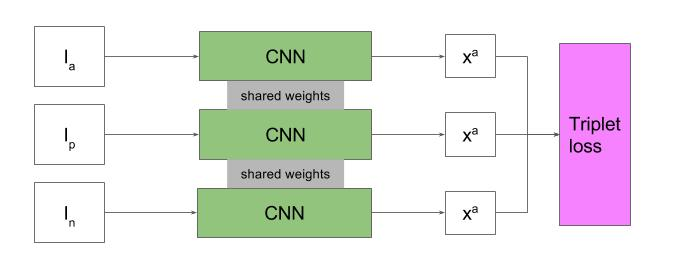
\includegraphics[width=\linewidth]{figures/3way_siamese__1_.jpg}
    \caption{Siamese Architecture use to train a network (NN) with a triplet of images, with an anchor image (a), a negative image (n) and a positive image (p)
    \label{fig:tripletloss}}
\end{figure}




%
%\section{Les visites augmentées}
%
%Système existant.
%Manière de tracker.
%
%
%\section{Instance, classe et identification}
%
%Difference entre recherche d'instance et classification
%Rechercher les travaux theorique sur la représentation d'instance.
%
%
%\section{Corpus d'images muséales}
%
%Il existe des collections sur des données muséales, comme le challenge du musée Rijk~\cite{mensink2014rijksmuseum}, qui propose plus de 110 000 œuvres artistiques du XIX$^{\text{\`e}me}$ siècle, ou le BNF Benchmark~\cite{picard2015challenges}. Cependant, ces corpus ne proposent qu'une seule image par œuvre et pas de requêtes adaptées à la recherche d'instances. Dans notre cas, plusieurs images par œuvre sont présentes et nous avons défini des requêtes associées. De plus, ces images ont des proportions variables d'arrière-plan, et sont prises de différentes perspectives.
%
%Les corpus d'images pour la recherche de catégorie d'objets (comme VOC 2007~\cite{Everingham2010} par exemple), ne sont pas adaptés à la recherche d'instance qui nous intéresse ici. La collection de la tâche {\it instance search} de TRECVid 2013\footnote{http://www-nlpir.nist.gov/projects/tv2013/tv2013.html\#ins} s'intéresse à des recherches d'instances, mais son corpus est uniquement composé de vidéos, ce qui sort du cadre de notre étude. Les caractéristiques des corpus qui se rapprochent des nôtres pour la recherche d'images au niveau instances sont à, notre connaissance, les suivants:
%\begin{itemize}
%\item Oxford Buildings\footnote{http://www.robots.ox.ac.uk/~vgg/data/oxbuildings/}: 5062 images, 55 requêtes, composée d'images représentant des bâtiments d'Oxford. Il y a 17 bâtiments différents, ce qui limite l'attrait pour la recherche d'instance. Ce corpus indique explicitement les images qui  portent partiellement sur un objet, ce qui peut permettre de mesurer la robustesse d'une approche. Des résultats publiés en 2015~\cite{Chatfield2015}  obtiennent des scores de MAP de 0.89, en concaténant cette collection avec un ensemble de 100 000 autres images tirées de Flickr, ce qui nous fait dire que cette collection n'est pas très difficile avec des approches de l'état de l'art;
%\item Holidays: 1491 images, 500 requêtes (scènes), composés d'images de vacances. Ce corpus contient quelques images par scène, et ne contient que des images en extérieur;
%\item Paris6k\footnote{http://www.robots.ox.ac.uk/~vgg/data/parisbuildings/}: 6412 images, avec des images de bâtiments parisiens. Ces images sont tirées de Flickr, donc peu contrôlées. Les autres caractéristiques sont similaires à Oxford5k;
%\item Sculpture6k\footnote{http://www.robots.ox.ac.uk/~vgg/data/sculptures6k/}: 6340 images (3170 de train et 3170 de test pour vérifier les modèles appris), 70 requêtes. Ce corpus est composé d'images de sculptures de Rodin et Moore. Les résultats reportés en 2011~\cite{Chatfield2015} par les auteurs de la collection donnent une MAP de 0,50, ce qui n'est pas très élevé. On peut donc considérer que cette collection est difficile, en particulier à cause de la nature 3D des œuvres considérées.
%\end{itemize}
%
%Le tableau~\ref{tab:exist_corpus} présente une description des collections ci-dessus dans le cadre de notre analyse de paramètres des collections.
%
%\begin{table}[htb]
%    \centering
%    \begin{tabular}{| c || c | c | c | c |}
%    \hline 
%    & Oxford5k & Holidays & Paris5k & Sculpture6k \\
%    \hline \hline
%    objet & bâtiments (3D) & scènes (3D) & bâtiments (3D) & œuvres (3D) \\
%    \hline 
%    support & Image & Image & Image & Image \\
%    \hline
%    acquisition & Flickr &  Flickr & Flickr & Flickr \\
%    \hline
%    taille (C/Q) &  5052 / 55 & 1491 / 500 & 6412 / 12& 6340 / 70\\
%    \hline
%    \end{tabular}
%    \caption{Caractéristiques des collections existantes}
%    \label{tab:exist_corpus}
%\end{table}
%
%Nous en concluons qu'il n'existe pas à notre connaissance de corpus d'objets de musées capables de représenter une certaine variabilité des objets (2D et 3D) et des supports (images ou vidéos), tout en garantissant un grand nombre d'images par objet recherché.
%
%
%\section{Descripteurs visuels locaux}
%
%Présenter les évolutions des descripteurs visuels.
%Ouvrir sur les réseaux de neurones
%
%
%\section{Réseaux de neurones à convolutions}
%
%Introduction au réseau de neurones.
%Comment on entraine une réseaux.
%Le besoin de données
%Les réseaux qui marchent le mieux.
%
%
%\section{Recherche d'instance à base de descripteurs visuels}
%Before the ground-breaking results of deep learning methods for object dection, and image retrieval, shallow descriptors like SIFT~\cite{lowe2004distinctive} have been used. Inspired by text retrieval methods like bag of words~\cite{barroso2003web}, methods used bag-of-features image representation~\cite{sivic2003video}. Each image is represented by a bag-of-features (BoF), with SIFT features clustered as vocabulary. For image retrieval, a inverted file structure~\cite{witten1999managing} is used to allow fast retrieval. An image is retrieved by computing its vector of visual words, and finding the closest one (by cosine distance).
%Aggregated descriptors like VLAD~\cite{jegou2010aggregating} are an evolution of BoF, with smaller vocabulary, more adapted to large dataset.
%The advantage of these methods is that they are compatible with query expansion. Query extension improve performance of retrieval system~\cite{arandjelovic2012three}, ranking image for a given region by tf-idf, and averaging BoF corresponding to the region visual words with the query BoF.
%
%\section{Methodes à base de réseaux de neurones}
%
%Plus grosse partie normalement.
%Aller de l'extraction de features à Gordo.
%
%After the success of CNN for classification, they have been used for several tasks, including image retrieval, with solid performances. 
%The first and trivial approach is to use CNN as features generator. A state-of-the-art large CNN is trained on an unrelated image classification dataset (e.g. ImageNet~\cite{deng2009imagenet}).
%This CNN is then to generated image representation~\cite{sharif2014cnn, babenko2014neural}. For image retrieval, the distance between the query image and collection images is performed to evaluate similarity.
%These methods outperformed standard descriptor approaches, but stay below the state of the art. 